\documentclass[border=2pt, 12pt]{standalone}

\usepackage{fontspec}
    \setmainfont{Times New Roman}
\usepackage[dvipsnames]{xcolor}
\usepackage{amsmath}
\usepackage{siunitx}
\usepackage{tikz}
    \usetikzlibrary{calc, math}

\begin{document}

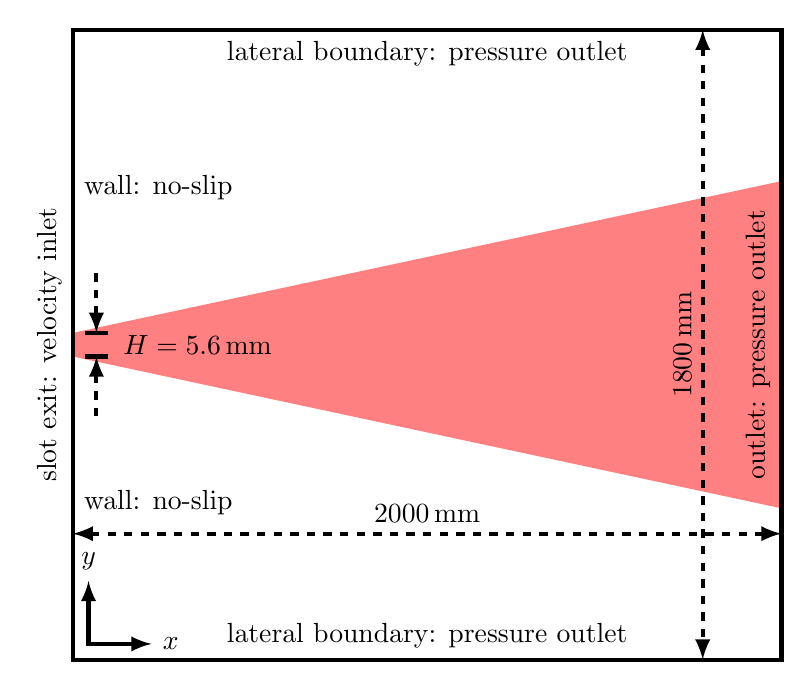
\begin{tikzpicture}[line width=1.5pt]
    \tikzmath{%
        \xlength=9;
        \ylength=8;
        \jetangle=13; % degree
    }
    \coordinate (A) at (0, 0);
    \coordinate (B) at (0, \ylength);
    \coordinate (C) at (\xlength, \ylength);
    \coordinate (D) at (\xlength, 0);
    \coordinate (O) at ($(A)!0.5!(B)$); % 射流出口中心点
    % 射流影响区域
    \fill [red!50] ($(O) + (0, 0.15)$) -- ($(O) + (\xlength, \xlength*tan \jetangle)$) -- ($(O) + (\xlength, -\xlength*tan \jetangle)$) -- ($(O) + (0, -0.15)$);
    % 边界框
    \draw (A) rectangle (C);

    % 坐标轴标识
    \draw [latex-latex] ($(A) + (0.2, 1)$) node [above] {$ y $} |- ($(A) + (1, 0.2)$) node [right] {$ x $};
    % 边界条件标识
    \node [above, rotate=90] at ($(O)$) {slot exit: velocity inlet};
    \node [right] at ($(A)!0.5!(O)$) {wall: no-slip};
    \node [right] at ($(O)!0.5!(B)$) {wall: no-slip};
    \node [above, rotate=90] at ($(C)!0.5!(D)$) {outlet: pressure outlet};
    \node [above] at ($(A)!0.5!(D)$) {lateral boundary: pressure outlet};
    \node [below] at ($(B)!0.5!(C)$) {lateral boundary: pressure outlet};
    % 尺寸标识
    \draw ($(O) + (0.15, -0.15)$) -- ++(0.3, 0);
    \draw [dashed, latex-] ($(O) + (0.3, -0.15)$) -- ++(0, -0.8);
    \draw ($(O) + (0.15, 0.15)$) -- ++(0.3, 0);
    \draw [dashed, latex-] ($(O) + (0.3, 0.15)$) -- ++(0, 0.8);
    \node [right=0.5cm] at (O) {$ H = \qty{5.6}{\mm} $};
    \draw [latex-latex, dashed] ($(A) + (0, 1.6)$) -- node [above] {$ \qty{2000}{\mm} $} ($(D) + (0, 1.6)$);
    \draw [latex-latex, dashed] ($(C) - (1, 0)$) -- node [above, rotate=90] {$ \qty{1800}{\mm} $} ($(D) - (1, 0)$);
\end{tikzpicture}

\end{document}